\documentclass[11pt,a4paper]{article}
\author{TalentSprint}
\date{}
\usepackage{verbatim}
\usepackage{fancyhdr}           % For header and footer
\usepackage{multicol}
\usepackage{colortbl}           % For coloured tables
\usepackage{setspace}           % For line height
\usepackage{seqsplit}           % Splits long words.
\usepackage{amsmath} 
\usepackage{graphicx}
\usepackage{array}
\usepackage{enumitem}
\usepackage{xcolor}
\usepackage[tikz]{bclogo}
\usepackage{textcomp}
\usepackage{listings}
\lstset{language=python,numbers=left,numberstyle=\tiny,numbersep=10pt,showstringspaces=false}

\headheight=14pt
\lhead{\nouppercase{}}
\rhead{\nouppercase{\leftmark}}

\graphicspath{{../Images/} {../ScreenShots/}}
\setcounter{tocdepth}{1}
\setlength\parindent{0pt}
\parskip=4pt
\newcommand{\Code}[1]{\textbf{\texttt{#1}}}

\begin{comment}
\def\AnswerBox{\fbox{\begin{minipage}{4in}\hfill\vspace{0.5in}\end{minipage}}}

\thispagestyle{empty}
\vspace{1.5pc}
\topskip0pt
\vspace*{\fill}
\centerline{\Huge Modern Programming}
\vspace{2pc}
\centerline{\Huge Practice}
\vspace{2pc}
\centerline{\Large using Python}
\vspace*{\fill}
\centerline{Prepared by TalentSprint WISE Team} 
\setcounter{page}{1}


\end{comment}
%========================================================================

% Lengths and widths
\addtolength{\textwidth}{5cm}
\addtolength{\hoffset}{-1cm}
\setlength{\headsep}{-12pt} % Reduce space between header and content
\setlength{\headheight}{85pt} % If less, LaTeX automatically increases it
\renewcommand{\footrulewidth}{2pt} % Remove footer line
\renewcommand{\headrulewidth}{1pt} % Remove header line
\renewcommand{\seqinsert}{\ifmmode\allowbreak\else\-\fi} % Hyphens in seqsplit
% This two commands together give roughly
% the right line height in the tables
\renewcommand{\arraystretch}{1.3}
\onehalfspacing



% Commands
\newcommand{\SetRowColor}[1]{\noalign{\gdef\RowColorName{#1}}\rowcolor{\RowColorName}} % Shortcut for row colour
\newcommand{\mymulticolumn}[3]{\multicolumn{#1}{>{\columncolor{white}}#2}{#3}} % For coloured multi-cols
\newcolumntype{x}[1]{>{\raggedright}p{#1}} % New column types for ragged-right paragraph columns
\newcommand{\tn}{\tabularnewline} % Required as custom column type in use

% Font and Colours
\definecolor{HeadBackground}{HTML}{333333}
\definecolor{FootBackground}{HTML}{666666}
\definecolor{TextColor}{HTML}{333333}
\definecolor{DarkBackground}{HTML}{6B8E23} %{FD1AA8}
\definecolor{LightBackground}{HTML}{E8FED8} %D3FDC8
\definecolor{tit}{HTML}{FF6600}
\renewcommand{\familydefault}{\sfdefault}
\color{TextColor}
 \headsep = 25pt
% Header and Footer
\pagestyle{fancy}
\usepackage[headheight=110pt]{geometry}
\fancyhf{}% Clear header/footer

\fancyhead[r]{
\includegraphics[width = 4cm, height = 2cm]{TS-Logo.png}\hspace{0cm}}

%=================================TITLE=====================================
\fancyhead[l]{\Large{\bf{\textcolor{tit}{\textrm{Dictionaries}}}}}
%===========================================================================

\renewcommand{\headrulewidth}{0.4pt}% Default \headrulewidth is 0.4pt
\renewcommand{\footrulewidth}{0.4pt}% Default \footrulewidth is 0pt

\rfoot{Page \thepage}
\lfoot{COPYRIGHT \textcopyright TALENTSPRINT, 2015. ALL RIGHTS RESERVED.}




\begin{document}



%\chapter*{Dictionaries}
A dictionary is one of the built-in function in Python, It is similar to list, but in dictionary the indices can be any type. It defines one-to-one relationships between keys and values.

\section*{Creating Dictionaries}
The function \emph{dict} creates a new dictionary with no items.
\begin{verbatim}
>>> name = dict()    # creates an empty dictionary with an variable name
>>> name
{}                   # represents an empty dictionary
\end{verbatim}
\begin{bclogo}[couleur=blue!5, arrondi=0.3, logo=\bctrombone]{Note}
\emph{dict} is a built-in function should not use as a variable name in Python.
\end{bclogo}

\section*{Adding items}
We use square brackets([]) to add items into the dictionary.
\begin{verbatim}
>>> name[`PCP'] = `C' # creates an item that maps from key `PCP'
                        to  the value  `C'
>>> print(name)       # It shows as a key-value pair with a colon between them
{`PCP':`C'}
\end{verbatim}
We can also create multiple items in a dictionary.
\begin{verbatim}
>>> name = {`PCP':`C', 	`MPP' = `Python', `OOPS':`Java'}
\end{verbatim}
\begin{figure}[ht]
\begin{center}
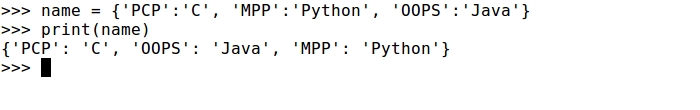
\includegraphics[scale=0.5]{Creating_Dictionaries.png}
\caption{Creating Dictionaries}
\label{Creating Dictionaries}
\end{center}
\end{figure}

\section*{Accesing Values}
We can access values from the dictionary as follows observe:
\begin{figure}[ht]
\begin{center}
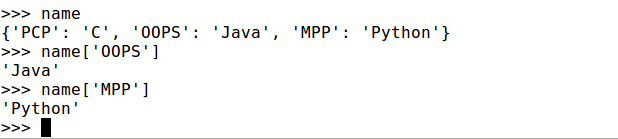
\includegraphics[scale=0.5]{Accessing_Values.png}
\caption{Accessing Values}
\label{Accessing Values}
\end{center}
\end{figure}

\section*{Modifying Dictionaries}
Assigning a value to an existing key  will wipe out the old value observe the following:
\begin{figure}[ht]
\begin{center}
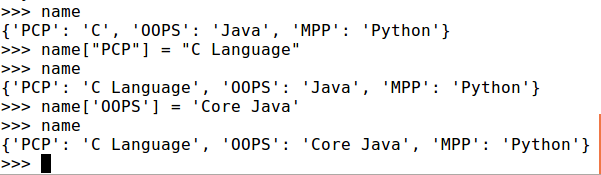
\includegraphics[scale=0.5]{Modifying_Dictionaries.png}
\caption{Modifying Dictionaries}
\label{Modifying_Dictionaries}
\end{center}
\end{figure}

\subsection*{Deleting items}
By using \emph{del} we can delete individual items from a dictionary by key.
\begin{figure}[ht]
\begin{center}
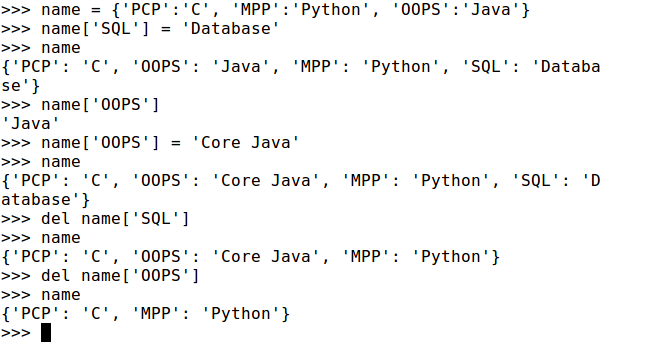
\includegraphics[scale=0.5]{Deleting_items.png}
\caption{Deleting Items}
\label{Deleting Items}
\end{center}
\end{figure}

\end{document}